\chapter{Nonlinear resonances} \label{app-A}


Following \cite{LundLecture1}, we return to one-dimensional motion and write
%
\begin{equation}\label{eq:Hill_nonlinear}
    x'' + k(s) x = \Delta B,
\end{equation}
%
where $\Delta B$ represents all the nonlinear terms in the expansion (and also linear deviations from the design fields). The stable solution $x_0$ when $\Delta B = 0$ is given by Eq.~\eqref{eq:Hill_solution}. We now define
%
\begin{equation}
    \phi(s) = \frac{1}{\nu} \oint{\frac{ds}{\beta(s)}},
\end{equation}
%
where $\nu$ is the tune. Moving to the normalized coordinate $u = x / \sqrt{\beta}$, with $\dot{u} = du/d\phi$ we have
%
\begin{equation}\label{eq:pert1}
    \ddot{u} + \nu^2 u = -\nu^2 \sum_{n=0}^{\infty}{\left(\beta^{\frac{n+3}{2}} b_{n+1}\right) u^n}.
\end{equation}
%
$\beta$ (the oscillation amplitude of the unperturbed motion) and $b_n$ (a multipole coefficient) are periodic in $\phi$ since they depend only on the position in the ring. Grouping these terms and Fourier expanding gives
%
\begin{equation}
    \ddot{u} + \nu^2 u = -\nu^2 \sum_{n=0}^{\infty}\sum_{k=-\infty}^{\infty} C_{n,k} \, u^n \, e^{ik\phi}.
\end{equation} 
%
We then perturb around $u_0$, the solution to the homogeneous equation, writing $u = u_0 + \delta u$, and keep only linear powers of $\delta u$. 
%
\begin{equation}
    \ddot{\delta u} + \nu^2 \delta u \approx -\nu^2 \sum_{n=0}^{\infty}\sum_{k=-\infty}^{\infty} C_{n,k} \, u_0^n \, e^{ik\phi}.
\end{equation}
%
Noting that
%
\begin{equation}
    u_0^n \propto \cos^n(\nu\phi) = \frac{1}{2^n}\sum_{m=0}^{n} \binom{n}{m} e^{i(n-2m)\nu\phi},
\end{equation} 
%
leads to
%
\begin{equation}\label{eq:pert2}
    \ddot{\delta u} + \nu^2 \delta u \approx -\nu^2 \sum_{n=0}^{\infty}\sum_{k=-\infty}^{\infty} \sum_{m=0}^{n} {n \choose m} \frac{C_{n,k}}{2^n} e^{i\left[(n - 2m)\nu + k\right]\phi}.
\end{equation}
%
A resonance condition may occur when any of the frequency components of the driving terms are close to the tune $\nu$; i.e., when
%
\begin{equation}
    (n - 2m)\nu + k = \pm \nu.
\end{equation}
%
Dipole terms correspond to integer tunes, quadrupole terms to 1/2 integer tunes, sextupole terms to 1/3 integer tunes, and so on. The same is true in the vertical dimension. The inclusion of coupling between $x$ and $y$ leads to the following resonance conditions:
%
\begin{equation}\label{eq:resonance_lines1}
    M_x \nu_x + M_y \nu_y = N,
\end{equation}
%
where $M_x$, $M_y$, and $N$ are integers and $|M_x| + |M_y|$ is the order of the resonance. These resonance lines are plotted in Fig.~\ref{fig:resonance_lines}.
%
\begin{figure}[!p]
    \centering
    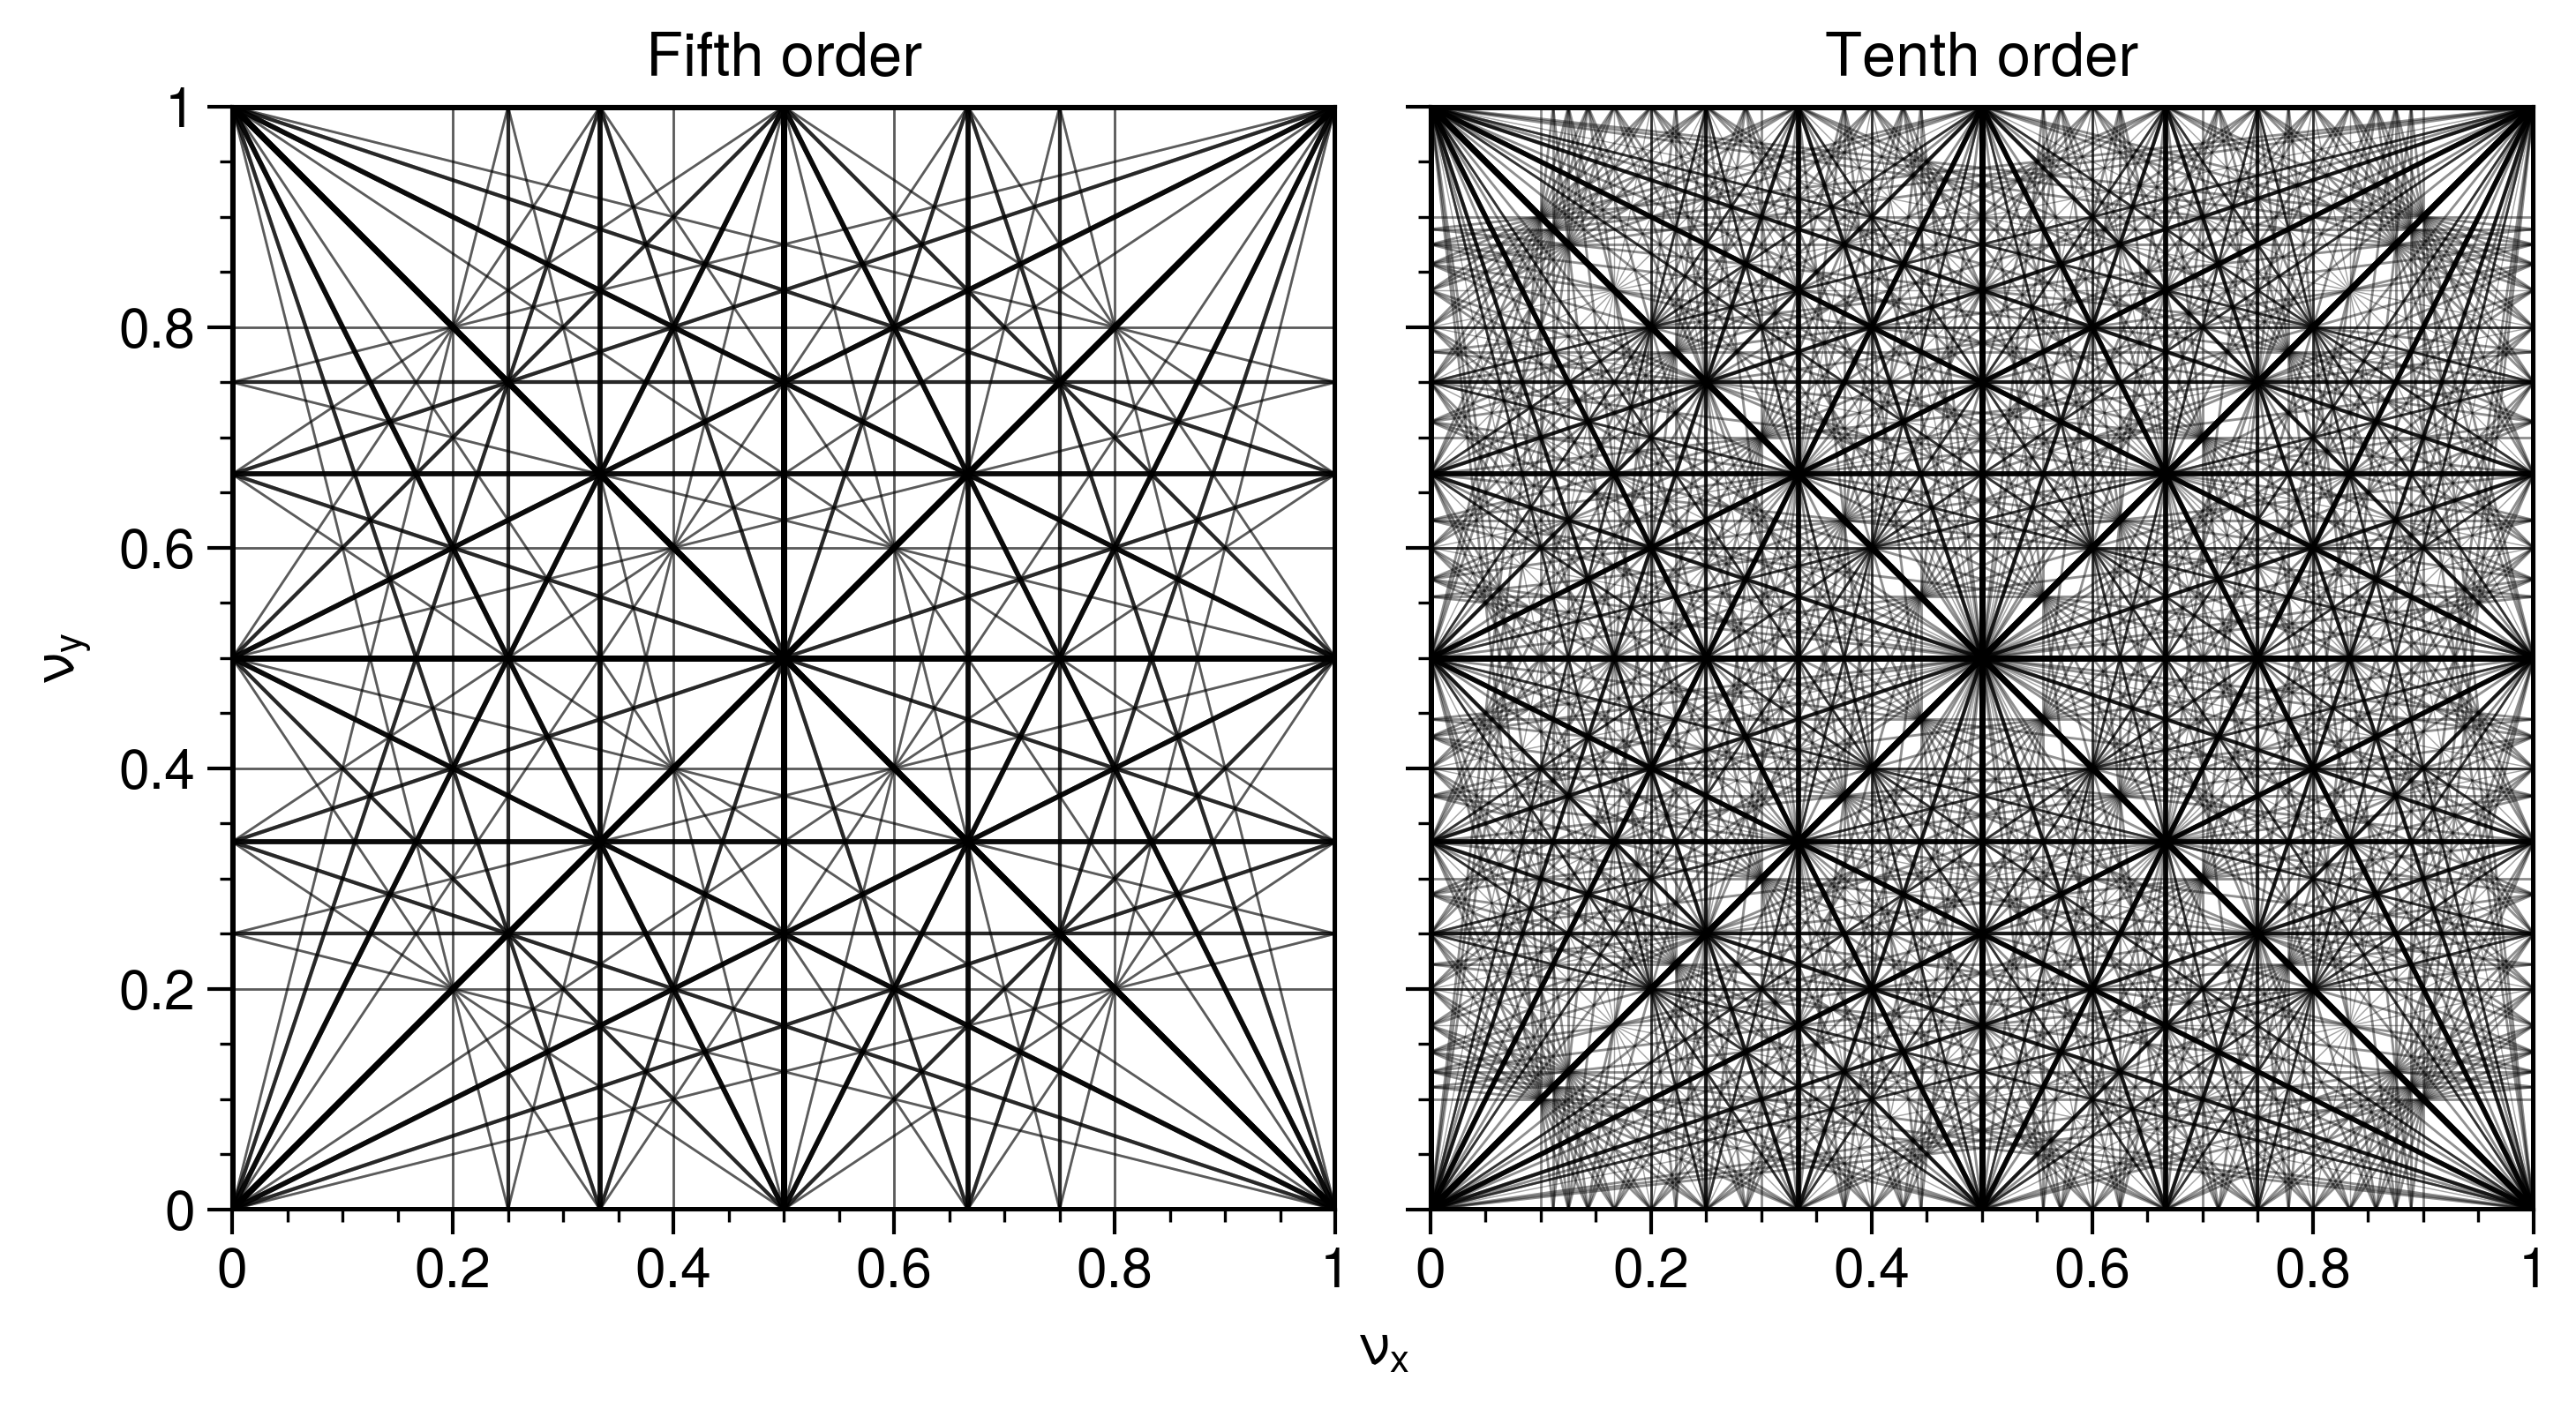
\includegraphics[width=\textwidth]{Images/chapter1/resonance_lines.png}
    \caption{Resonance lines in tune space defined by Eq.~\eqref{eq:resonance_lines1}.}
    \label{fig:resonance_lines}
\end{figure}
%
\begin{figure}[!p]
    \begin{subfigure}[b]{1.0\textwidth}
        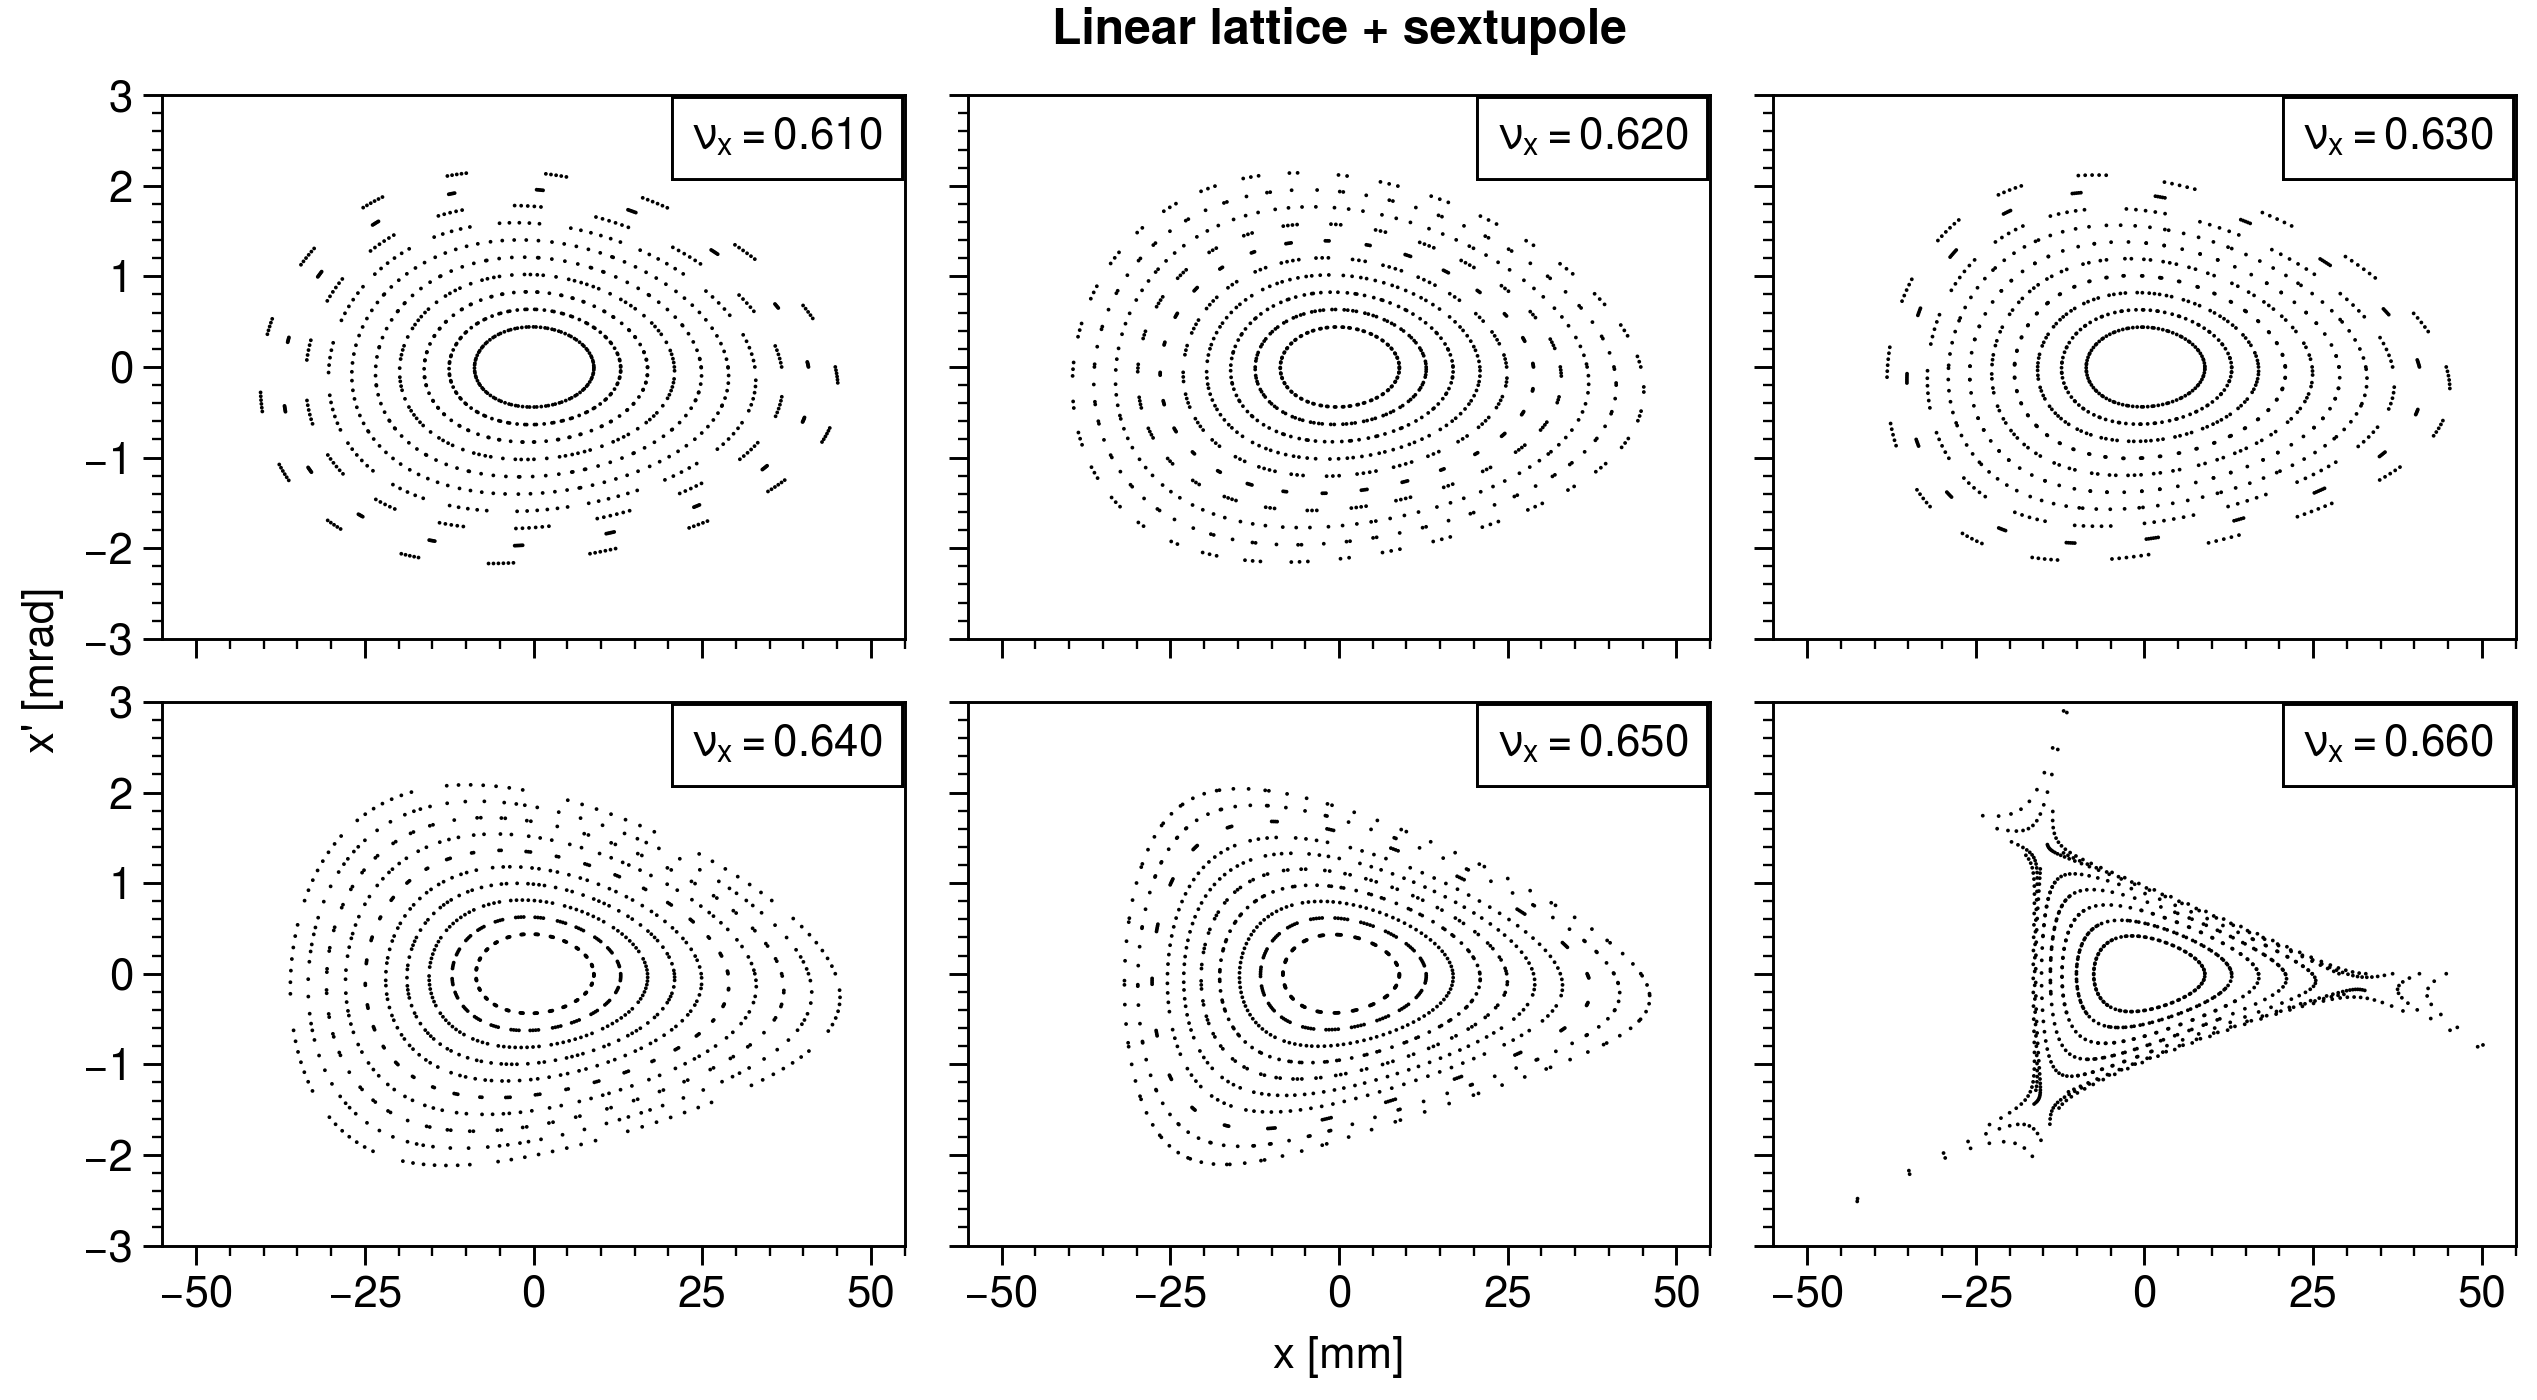
\includegraphics[width=\textwidth]{Images/chapter1/sextupole.png}
        \label{fig:sextupole_a}
    \end{subfigure}
    \vfill
    \vspace*{1.0cm}
    \vfill
    \begin{subfigure}[b]{\textwidth}
        \centering
        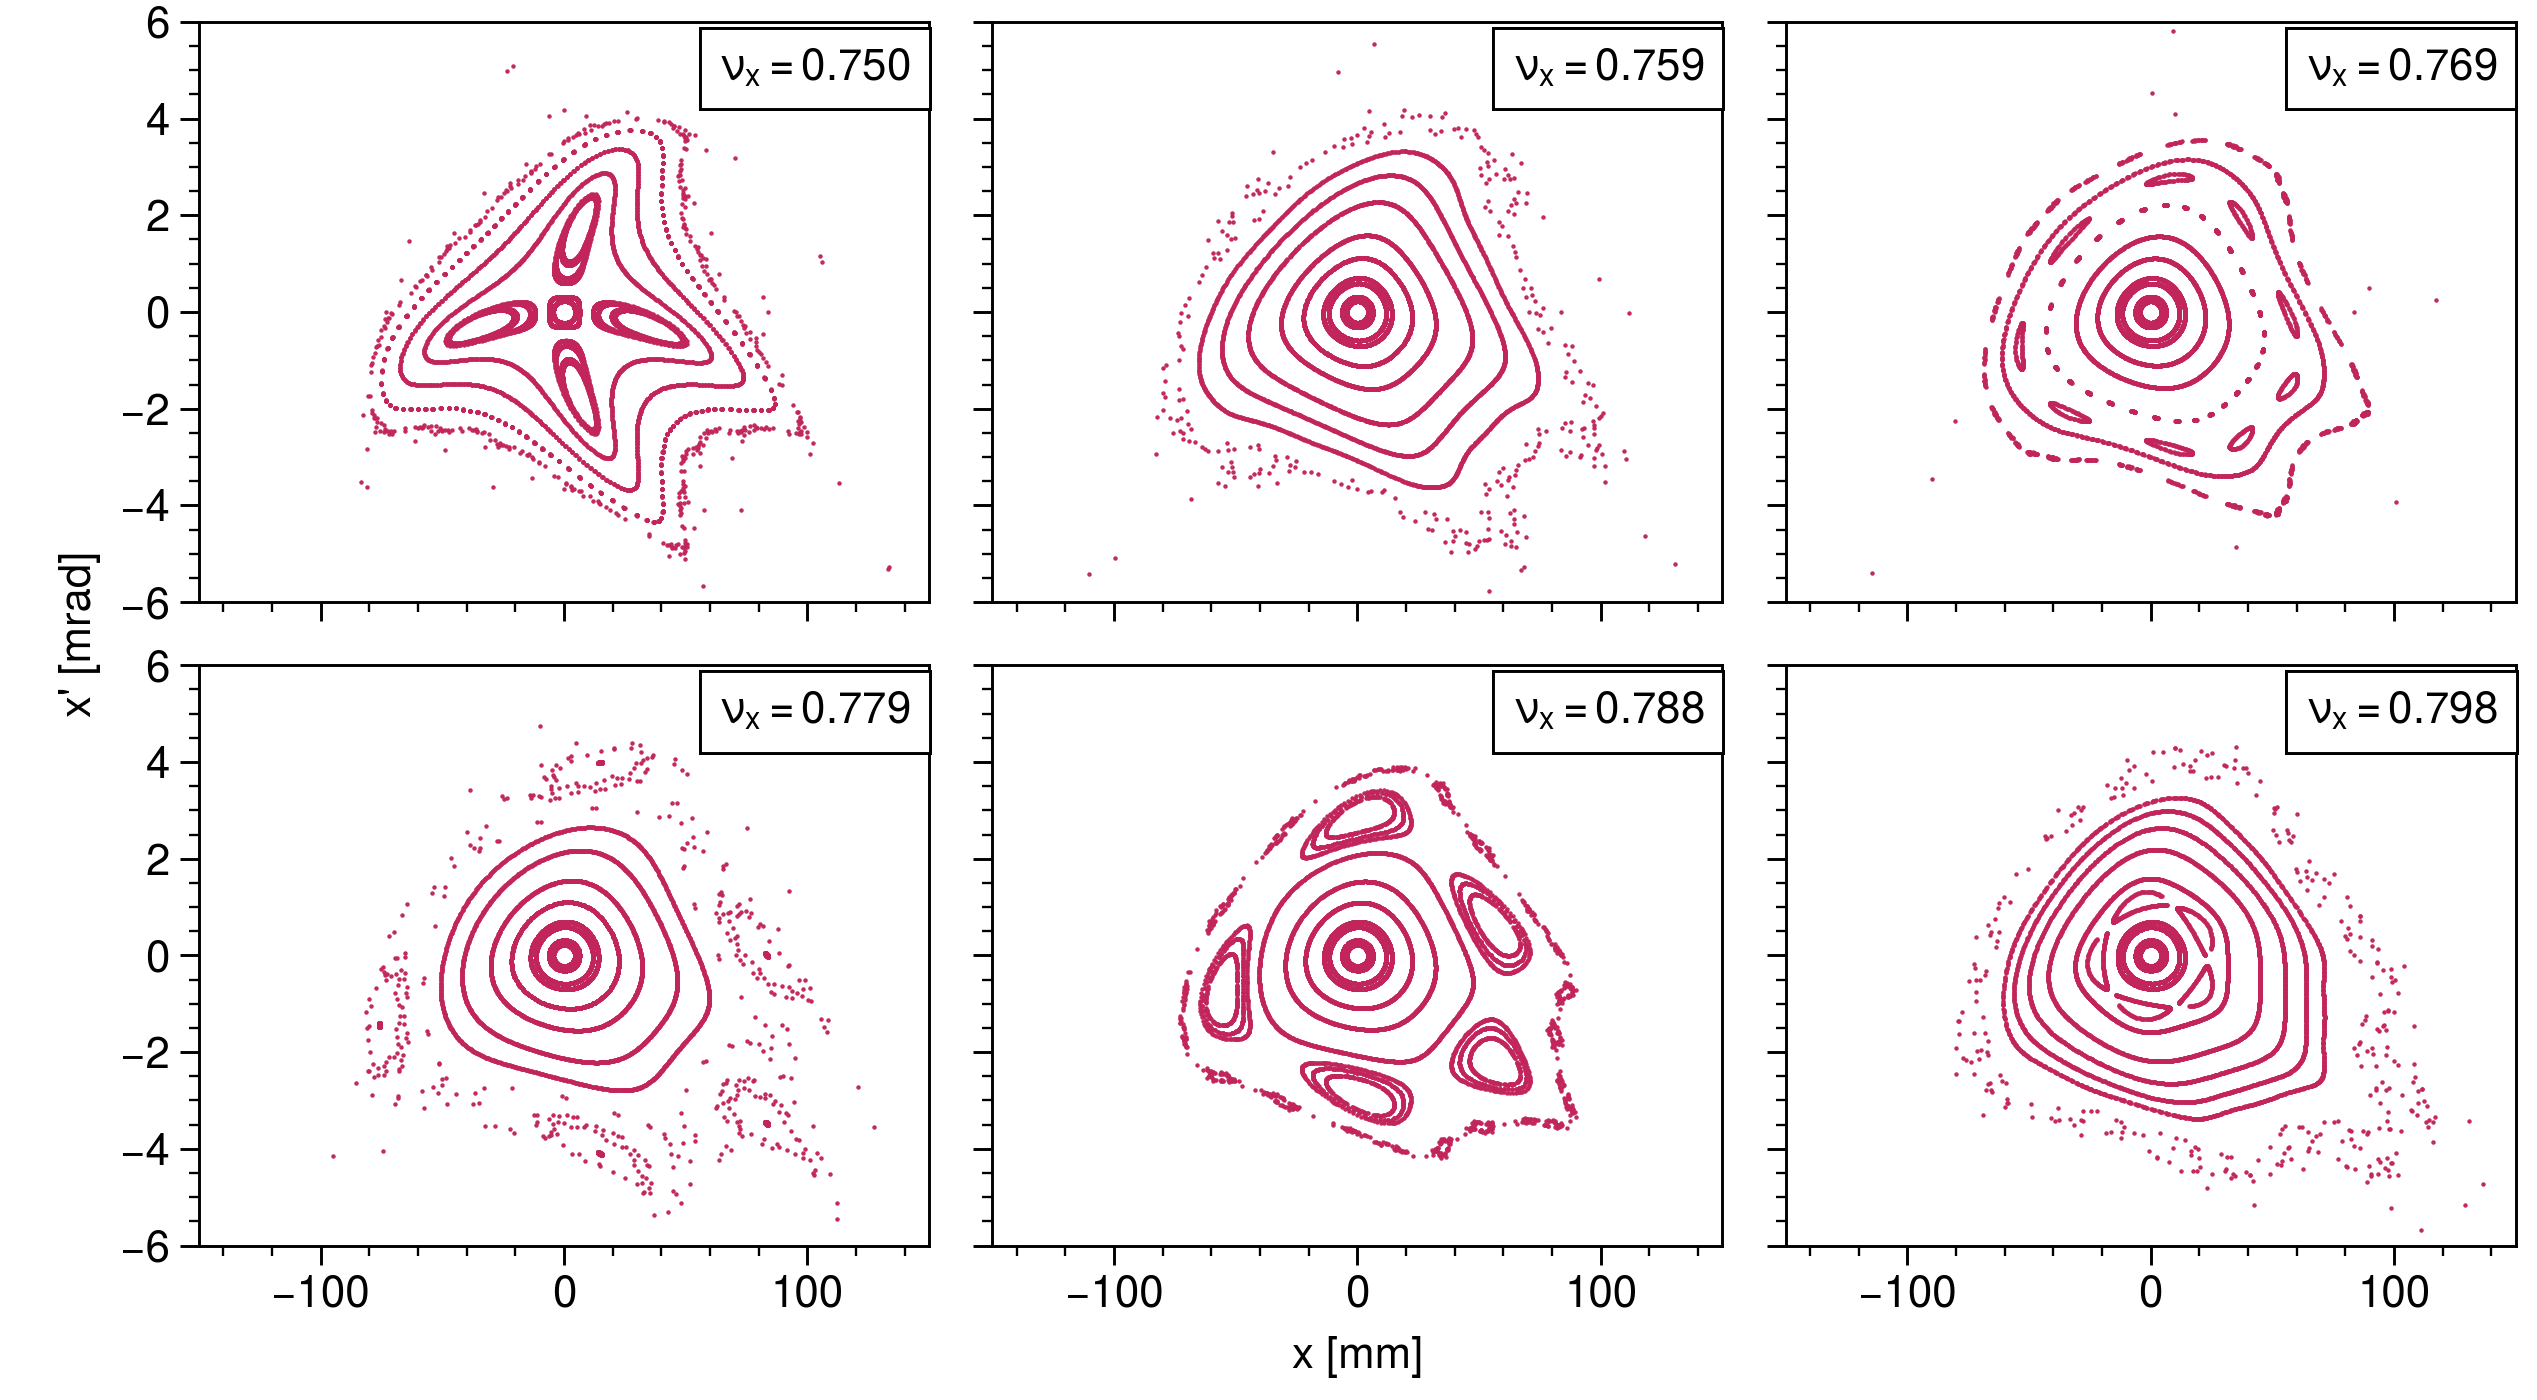
\includegraphics[width=\textwidth]{Images/chapter1/sextupole_second_order.png}
        \label{fig:sextupole_b}
    \end{subfigure}
    \caption{Third-order (top) and fourth/fifth-order (bottom) resonances excited by a sextupole perturbation to a linear lattice. (Adapted from \cite{Lee2011}.)}
    \label{fig:sextupole}
\end{figure}
%
The strength of the resonance varies inversely with the order; fourth-order and below are the primary concern in most machines, but higher-order effects may be important when the number of stored turns is large. 

Nonlinear dynamics can be studied using mapping equations \cite{Reichl1992}. For illustration, Fig.~\ref{fig:sextupole} shows two numerical experiments from \cite{Lee2011} involving a sextupole perturbation to an otherwise linear lattice. The turn-by-turn trajectories of particles with several different initial amplitudes are plotted for different tunes $\nu_x$. The third-order resonance leads to a well-known triangular region of stability as the tune approaches 2/3. The bottom plot reveals fourth and fifth-order resonances only obtained from second-order perturbation analysis.